\documentclass{beamer}
\usepackage[utf8]{inputenc}
\usepackage[T1]{fontenc}
\usepackage{mathabx}
\usepackage{mathpazo}
\usepackage{eulervm}
\usepackage{natbib}

%\usetheme{Pittsburgh}
\usetheme{Boadilla}
\usefonttheme{professionalfonts}
\usecolortheme{wolverine}
%\useoutertheme{miniframes}
%\setbeamertemplate[miniframes theme]{headline}


\title{VP160: Honors Physics I}
\subtitle{TA Workshop}
\author{Zeyi Ren}
\institute{UM-SJTU Joint Institute}

\begin{document}

\maketitle

\frame{\tableofcontents}

\section{Professor \& TAs}
\begin{frame}{Professor \& TAs}
    %Mateusz Krzyzosiak
    \begin{figure}[T]
        \centering
        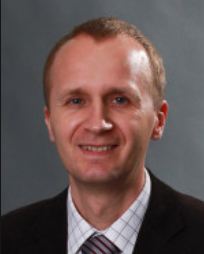
\includegraphics[width=0.2 \linewidth, angle =0]{mk.png}
      \end{figure}
      \centering{Mateusz Krzyzosiak}
      \begin{itemize}
        \item Kind and cute, very easy-going.
        \item Teach VP150, VP160, VP390.
        \item Good English.
      \end{itemize}
      \flushleft{TAs:}
      \begin{itemize}
        \item Pingchaung Ma \quad \textit{hensonma@sjtu.edu.cn} 
        \item Zeyi Ren \quad\quad\quad\quad \textit{renn\_08@sjtu.edu.cn}
      \end{itemize}
\end{frame}
\section{Course Content}
\begin{frame}{Course Content}
    \begin{enumerate}
        \item Kinetics in 3D
        \item Newton's Law
        \item Harmonic Oscillation (*detailed calculation for damped system)
        \item Non inertia FOR (circular motion under spheric coordinates)
        \item Work and kinetic energy
        \item *Lagrangian Mechanics
        \item Momentum
        \item Rigid body dynamics (*moment of inertia tensor)
    \end{enumerate}
    \textbf{What's different from VP150?}\\
    \begin{itemize}
      \item 20\% more content (*)
      \item More fundamental start point (Basic theories $\to$ Detailed calculation and derivation $\to$ Results)
      \item Deeper understanding of Physics.
    \end{itemize}
\end{frame}

\section{Workload}
\begin{frame}{Workload}
  \begin{itemize}
    \item 1 homework per week (3-4 hrs), 12 in total, less than VP150.
    \item 1 term project $\approx $ 2.5 hw (4-5 person per group, self grouping).\\Last year: \underline{\small{\url{https://jbox.sjtu.edu.cn/l/yF3W6g}}}
    \item Some time for review and self learning.
  \end{itemize}
  ~\\
  \centering
  VP160 workload $\gg $ VP150 workload? No.
  \end{frame}

\section{About Grading}
\begin{frame}{About Grading}
  From Last year:
  \begin{itemize}
    \item Homework 25\% =  12 problem sets 25\%$\times $75\% + 1 term project 25\% $\times $25\%
    \item Online activities 15\% (last year in class quiz, this year possibly not).
    \item 1 Mid 30\%
    \item 1 Final 30\%
  \end{itemize}
    Syllabus for last year: \underline{\small{\url{https://jbox.sjtu.edu.cn/l/KFggnC}}}\\
    ~\\
    Better grading, the expected median grade is "$B^+$".\\
    Why? A larger chance of getting an "$A$" or "$A^+$".
    \end{frame}

\section{How to learn VP160 well?}
\begin{frame}{How to learn VP160 well?}
    \begin{itemize}
      \item Never fight alone! Don't stuck on one problem for too much time, don't waste your amazing life! Ask your great fellow classmates (I bet some of you are masters of Physics), your TAs and MK for help. Don't be shy!
      \item Follow MK during lectures! Try to understand the relationship between physics principles rather than copying the notes.
      \item Choose a cozy time to attend RCs.
      \item Take problem sets seriously. Doing some exercises is the best way to learn physics.
      \item If you feel panic or left behind, OHs are there for you (face-to-face meetings would be recommended).
    \end{itemize}
\end{frame}

\begin{frame}
  Generally speaking, the course materials are enough for you to learn very well, but if you have time, here is a useful book :)\\
  \underline{\small{\url{https://jbox.sjtu.edu.cn/l/uFljNn}}}
\end{frame}
\begin{frame}
  \centering
  \huge{Have fun!!!}\\
  \huge{Q \& A}
\end{frame}
\renewcommand{\bibfont}{\footnotesize}
\frametitle{Bibliography}

\bibliographystyle{apalike}
\bibliography{refs}

% \end{frame}


\end{document}
